\section{The Arrival Transient}
\label{sec:transient}

Before looking at any data we can work out what should happen in the first steps after a reduced state arrives.
It takes nothing more than \eqref{eq:m}--\eqref{eq:step}, and the answer tells us which strategies are worth running
and what to expect from each. Number the steps after
arrival $k = 1, 2, \dots$ and consider one coordinate whose gradient over this short window has mean $\mu$ and variance
$\sigma^2$, with independent noise from step to step. Let $R(k)$ be the root-mean-square size of the update at step
$k$ divided by its size in the uninterrupted run. Two limits bracket the behaviour: a coordinate dominated by noise
($\mu = 0$) and one dominated by signal ($\sigma = 0$). In the uninterrupted run the noise-dominated update has
size $\eta\sqrt{(1-\beta_1)/(1+\beta_1)}$, about $0.23\,\eta$ at $\beta_1 = 0.9$, and the signal-dominated one has
size $\eta$. The Adam counter at arrival is large, so that both bias corrections equal one unless the counter is reset.

\begin{proposition}[Size of the arrival transient]
\label{prop:transient}
Approximating $v$ by its expectation, the update inflation $R(k)$ is as follows.

\smallskip
\noindent\small\setlength{\tabcolsep}{3pt}\begin{tabular}{@{}lll@{}}
\toprule
State on arrival & Noise-dominated & Signal-dominated \\
\midrule
$m = v = 0$, counter kept & $\sqrt{\dfrac{1-\beta_1^{2k}}{1-\beta_2^{k}}}$ & $\dfrac{1-\beta_1^{k}}{\sqrt{1-\beta_2^{k}}}$ \\[2.2ex]
$m = v = 0$, counter reset & $\sqrt{\dfrac{1+\beta_1^{k}}{1-\beta_1^{k}}}$ & $1$ \\[2.2ex]
$m = 0$, $v$ carried & $\sqrt{1-\beta_1^{2k}}$ & $1-\beta_1^{k}$ \\[1.2ex]
$m$ carried, $v = 0$ & $1/\sqrt{1-\beta_2^{k}}$ & $1/\sqrt{1-\beta_2^{k}}$ \\
\bottomrule
\end{tabular}
\end{proposition}

\begin{IEEEproof}
From \eqref{eq:m} with $m_0 = 0$, $m_k = (1-\beta_1)\sum_{i \le k} \beta_1^{k-i} g_i$, so
$\mathbb{E}\,m_k = (1-\beta_1^k)\mu$ and
$\operatorname{Var} m_k = \frac{1-\beta_1}{1+\beta_1}(1-\beta_1^{2k})\sigma^2$; likewise
$\mathbb{E}\,v_k = (1-\beta_2^k)(\mu^2+\sigma^2)$ from \eqref{eq:v}. A carried moment keeps its stationary value. Rows one,
three and four are ratios of these to the stationary values. Resetting the counter divides $m_k$ by $1-\beta_1^k$ and
$v_k$ by $1-\beta_2^k$, which gives row two. At $k = 1$ the first row is exact, with no approximation: the update is
$\eta\,(1-\beta_1)/\sqrt{1-\beta_2}$ times the sign of the gradient on every coordinate.
\end{IEEEproof}

Four consequences follow, and the experiments test each of them.

\textbf{The first update after a cold arrival is large, not small.} With $\beta_1 = 0.9$ and $\beta_2 = 0.99$ a
noise-dominated coordinate moves $\firstNoiseA$ times further than it would have; with $\beta_2 = 0.999$,
$\firstNoiseB$ times. The intuition that zeroed moments give a near-zero first step holds only for optimizers that
apply the step before updating the moments.

\textbf{Keeping the step counter makes a cold arrival worse.} With the counter kept, the inflation in row one decays as
$1/\sqrt{1-\beta_2^k}$, on the horizon of the \emph{second} moment: the excess movement, $\sum_k (R(k)-1)$, grows in
proportion to $1/(1-\beta_2)$ and is \excessZerosC{} steps' worth at $\beta_2 = 0.95$, \excessZerosA{} at $0.99$
and \excessZerosB{} at $0.999$. With the counter
reset, the bias correction supplies exactly the factor that $v$ lacks, the inflation decays on the horizon of the
\emph{first} moment, and the excess is \excessFreshA{} steps' worth at any $\beta_2$. In the signal-dominated limit
the kept counter overshoots by up to \overshootA{} at step \overshootAtA{} (\overshootB{} for $\beta_2 = 0.999$) where
the reset counter does not overshoot at all. A reset is the right companion to an empty optimizer, and the wrong one to
a carried moment.

\textbf{The first moment is cheap to lose.} With $v$ intact and $m$ refilling from zero the update is too
\emph{small}, by $\sqrt{1-\beta_1^{2k}}$, and only for about $1/(1-\beta_1)$ steps. The shortfall sums to
\deficitM{} steps of progress. Nothing can diverge. This is why every strategy in the middle family drops $m$.

\textbf{The second moment must never be the only thing missing.}

\begin{corollary}
\label{cor:wm}
If $m$ is carried and $v$ is zeroed with the counter kept, the first update is at least $1/\sqrt{1-\beta_2}$ times the
steady one in root-mean-square, and its norm is dominated by coordinates whose current gradient happens to be small.
\end{corollary}

\noindent The carried $m$ is divided by $\sqrt{(1-\beta_2)}\,|g_1|$, and $m$ is independent of $g_1$, so a coordinate
with a small $|g_1|$ takes an arbitrarily large step. When both moments are zeroed this cannot happen, because $m_1$ is
then proportional to the same $g_1$. We run \arm{w\_m} as the measured counterpart of this statement; the
strategy validator otherwise rejects it.

The proposition also says what the sketch of $v$ has to preserve. Only $\sqrt{v}$ enters the step, coordinate by
coordinate; a sketch that gets its scale right within a tensor moves the update by the relative error of $\sqrt{v}$,
not by an order of magnitude, and the error is forgotten on the horizon $1/(1-\beta_2)$ as true squared gradients
arrive.

\begin{figure}[t]
\centering
\IfFileExists{gen/figures/trace.pdf}{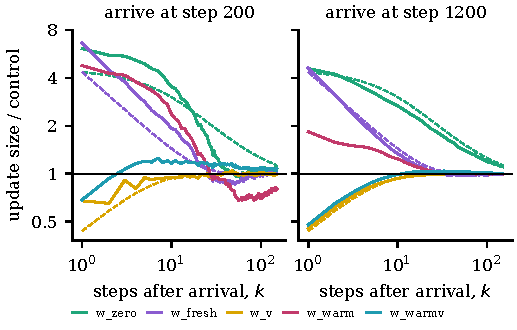
\includegraphics[width=\columnwidth]{trace}}{}
\caption{Size of each update after arrival, divided by the size of the same update in the uninterrupted run
(\traceScale, mean of \traceSeeds{} seeds). Dashed lines are the noise-dominated column of
Proposition~\ref{prop:transient}, with no fitted parameter.}
\label{fig:trace}
\end{figure}

\textbf{Measured update sizes.} Fig.~\ref{fig:trace} overlays the prediction on the measured size of every update for
the first \traceSteps{} steps after arrival.
At 60\% of the schedule the closed forms follow the measurement from the first step to the last. With both moments
zeroed and the counter kept, the first update is \traceZeroOne{} times the control's (predicted \predZeroOne), the
tenth \traceZeroTen{} (\predZeroTen) and the hundredth still \traceZeroHundred{} (\predZeroHundred). With the counter
reset the first update is the same size, \traceFreshOne, and the tenth is down to \traceFreshTen{} (\predFreshTen);
by the hundredth it is \traceFreshHundred. With only $m$ dropped the first update is \traceVOne{} of the control's
(\predVOne) and the tenth \traceVTen{} (\predVTen); the rank-one sketch of $v$ gives \traceRankOne{} and
\traceRankTen, indistinguishable from the exact $v$, and the quantised moments give \traceQOne{} throughout.
At 10\% of the schedule, where the learning rate is at its peak and the loss is still falling fast, the gradient is not
pure noise and the weights move during the transient; the initial inflation is larger than the noise-dominated
value (\traceZeroOneEarly{} and \traceFreshOneEarly) and the run with the kept counter falls back to the control's
step size sooner than predicted, after the damage of Section~\ref{sec:fork} is done. The ordering of the strategies is
the same at both points.


\textbf{A first moment cannot be re-estimated at a point.} The \arm{warm} rule rebuilds $m$ as the mean of
\warmPasses{} gradients at the arrival weights. Under the model above this would have nearly the same size as the
carried $m$, since averaging \warmPasses{} independent gradients removes about as much noise as the exponential average
does. It does not: the rebuilt $m$ is \mnormWarm{} times larger than the one left behind (Section~\ref{sec:diag}). The
model's assumption of independent gradients is what fails. Along a training trajectory successive gradients are
anti-correlated in the directions of high curvature, where adaptive methods oscillate~\cite{cohen2022aeos}, and the
exponential average cancels them. Gradients taken repeatedly at one point all contain that component with the same
sign. The moment $m$ is therefore a statistic of the trajectory and not of the point where it stopped, and an estimate
made at a standstill overstates it. Squared gradients do not cancel, so $v$ can be re-estimated at a point; that is
the \arm{warmv} rule.
